\begin{flushleft}
\section{\LARGE{Opis techniczny}}
\end{flushleft}

\begin{flushleft}
    \subsection{\Large{Narzędzie}}
    \hspace{5mm}Do tworzenia aplikacji \textquotedbl Szpital+\textquotedbl{} korzystałem z narzędzi {\color{blue}\href{https://pl.wikipedia.org/wiki/Windows_Presentation_Foundation}{WPF(Windows Presentation Foundation)}}. Jest to narzędznie do trowrzenia aplikacji desktopowych dla systemów Windows na bazie {\color{blue}\href{https://pl.wikipedia.org/wiki/.NET_Framework}{.Net Framework}}. Wykorzystywuje język opisy interfejsu użytkownika({\color{blue}\href{https://pl.wikipedia.org/wiki/Extensible_Application_Markup_Language}{XAML}}\label{href:XAML}) oraz język programowania {\color{blue}\href{https://pl.wikipedia.org/wiki/C_Sharp}{C\#}}\label{href:c_sh} do implementacji funkcjonalności elementów i innych funckji backend.
    \\
    \hspace{5mm} Dodatkowo przestrzegałem {\color{blue}\href{https://en.wikipedia.org/wiki/Model%E2%80%93view%E2%80%93viewmodel}{wzóru architektonicznego MVVM}}(Model-View-ViewModel)\label{href:MVVM}. Jest to wzór który rozdziela graficzny interfejs użytkownika GUI(View) od implementacji logiki biznesowej oraz logiki backend. Związkiem między tymi warstami jest konwerter wartości (ViewModel), który przyjmuje publiczne właściwości modeli(Models) i przekazuje ich do widoków(Views) za pomocą wiązania (Binding).
    \\
    \hspace{5mm} Do pisania kodu korzystałem z środowiska programistycznego {\color{blue}\href{https://pl.wikipedia.org/wiki/Microsoft_Visual_Studio}{Microsoft Visual Studio}\label{href:VStudio}}.
    \\
    \hspace{5mm}Także wykorzystełem wtyczki \textquotedbl {\color{blue} \href{https://github.com/charri/Font-Awesome-WPF}{FontAwesome.WPF}}\textquotedbl{} dla dodania ikon jako tekstu dla nawigacji bocznej i wtyczki \textquotedbl {\color{blue}\href{https://github.com/dotnet/corefx}{System.Data.SqlClient}}\textquotedbl{} dla połączenia z bazą danych SQL.
\end{flushleft}

\begin{flushleft}
    \subsection{\Large{Minimalne wymagania sprzętowe}}
    \begin{itemize}
        \item System operacyjny: Microsoft Windows 10 lub wyżej
        \item Procesor: x86 lub x64 z szybkością > 800 MHz
        \item RAM: 512 MB
        \item Miejsca na dysku: 25 MB
        \item Zainstalowany .Net 8.0
    \end{itemize}
\end{flushleft}

\begin{flushleft}
    \subsection{\Large{Baza danych}}
    \hspace{5mm}Do stworzenia i zarządzania bazą danych wykorzystywałem {\color{blue}\href{https://en.wikipedia.org/wiki/SQL_Server_Management_Studio}{Microsoft SQL Server Management Studio}}. Na lokalnym serwerze stworzyłem bazę danych "Spzital" (Rys.~\ref{fig:db_diag}). Także uzupełniłem bazę losowymi wartościami i dodałem kilka ograniczeń. Na przykład ograniczenie na wprowadzenie do nr\_grabinetu w wizycie większego od 127.
    \begin{figure}[H]
	\begin{center}
	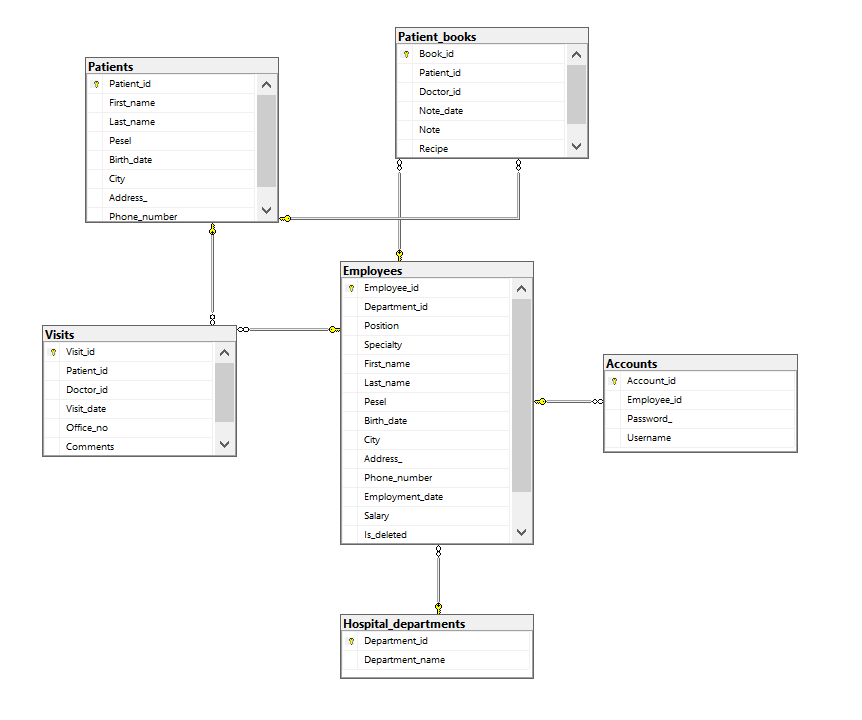
\includegraphics[width=10cm, height=10cm]{images/db_diagram.png}
        \caption{Diagram bazy danych}
        \label{fig:db_diag}
	\end{center}
    \end{figure}
    
    \hspace{5mm} Do pobrania danych z bazy do aplikacji wykorzystywuję klasy statycznej DbContext(Rys.~\ref{fig:db_c_k}) w której są metody robiące zapytania na bazę danych i wracające wartości pobrane z bazy.
    \begin{figure}[H]
    \centering
    \subfigure{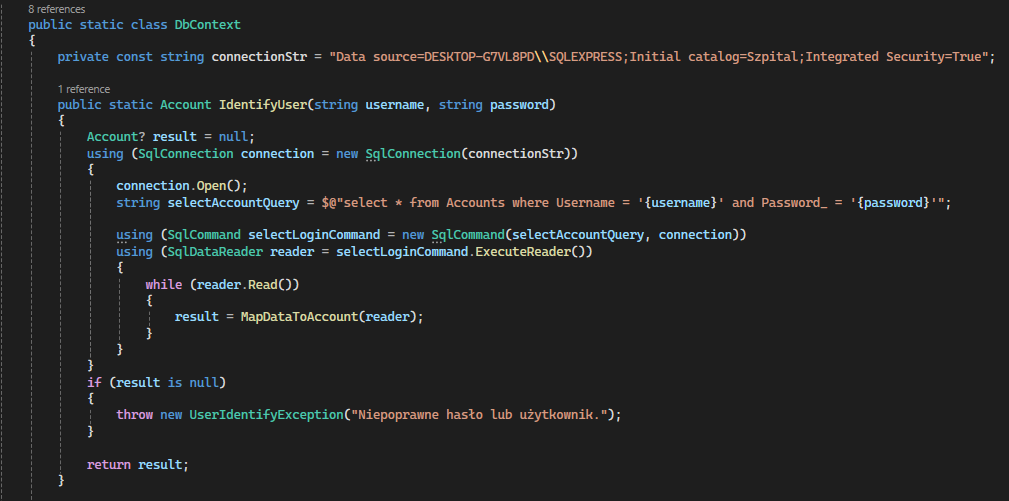
\includegraphics[width=0.6\textwidth]{images/db_cont_klas1.png}} 
    \subfigure{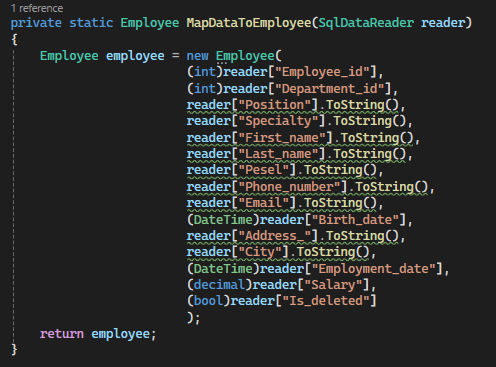
\includegraphics[width=0.38\textwidth]{images/db_cont_klas2.png}} 
    \caption{Klasa do zarządzania bazą danych(Przykładowa metoda)}
 
    \label{fig:db_c_k}
    \end{figure}
\end{flushleft}